\section{Mine-sweeper}
\tikzstyle{vertex}=[auto=left,circle,fill=black!25,minimum size=20pt,inner sep=0pt]

\textbf{Proof:} 
\begin{itemize}
	\item Certificate: Given such a graph, we can verify whether a node $v$ that is labeled $m$ has exactly $m$ neighboring nodes containing mines in polynomial time, thus it is a NP problem;
	\item NP-hard: Now we prove that $3-SAT \leq_p Mine-consistency$. \\
	For instance,if a clause of $3-SAT$ is $ x_1 \vee \neg x_2 \vee  x_3 $,then we can construct a graph 
		\begin{center} 
			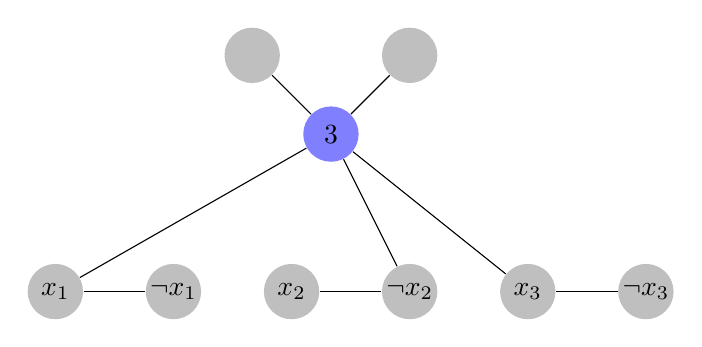
\begin{tikzpicture}
			\node[vertex] (s1)  at (1,4)  {};
			\node[vertex] (s2)  at (3,4)  {};
			\node[vertex,fill = blue!50] (s3)  at (2,3)  {3};
			
			\node[vertex] (x1) at(-1.5,1) {$x_1$};
			\node[vertex] (x1') at(0,1) {$\neg x_1$};
			\node[vertex] (x2) at (1.5,1) {$x_2$};
			\node[vertex] (x2') at (3,1) {$\neg x_2$};
			\node[vertex] (x3) at (4.5,1) {$x_3$};
			\node[vertex] (x3') at (6,1) {$\neg x_3$};
			\draw (s1) -- (s3);
			\draw (s2) -- (s3);
			\draw (s3) -- (x1);
			\draw (s3) -- (x2');
			\draw (s3) -- (x3);
			\draw (x1) -- (x1');
			\draw (x2) -- (x2');
			\draw (x3) -- (x3');
			\end{tikzpicture}
		\end{center} 
	If node $v$ has a mine ,we color it \textit{red}, otherwise we color it \textit{green}.If $3-SAT$ is satisfied, then we can color the neighboring nodes of blue node $3$ to make sure that blue node $3$ has exactly $3$ neighboring nodes containing mines. For instance, if $x_1 = 1, x_2 = 1, x_3 = 0$,then we color the graph 
		\begin{center} 
			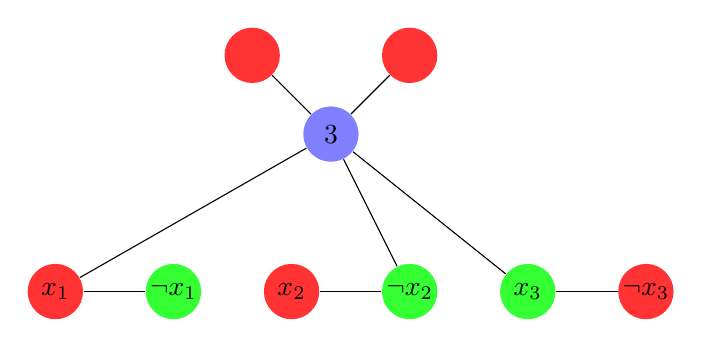
\begin{tikzpicture}
			\node[vertex, fill = red!80] (s1)  at (1,4)  {};
			\node[vertex, fill = red!80] (s2)  at (3,4)  {};
			\node[vertex,fill = blue!50] (s3)  at (2,3)  {3};
			
			\node[vertex, fill = red!80] (x1) at(-1.5,1) {$x_1$};
			\node[vertex, fill = green!80] (x1') at(0,1) {$\neg x_1$};
			\node[vertex,fill = red!80] (x2) at (1.5,1) {$x_2$};
			\node[vertex, fill = green!80] (x2') at (3,1) {$\neg x_2$};
			\node[vertex, fill = green!80] (x3) at (4.5,1) {$x_3$};
			\node[vertex,fill = red!80] (x3') at (6,1) {$\neg x_3$};
			\draw (s1) -- (s3);
			\draw (s2) -- (s3);
			\draw (s3) -- (x1);
			\draw (s3) -- (x2');
			\draw (s3) -- (x3);
			\draw (x1) -- (x1');
			\draw (x2) -- (x2');
			\draw (x3) -- (x3');
			\end{tikzpicture}
		\end{center} 	
	if the clause $x_1 \vee \neg x_2 \vee x_3$ is \textit{False}, which means that $x_1 = 0, x_2 = 1, x_3 = 0$, then 
		\begin{center} 
			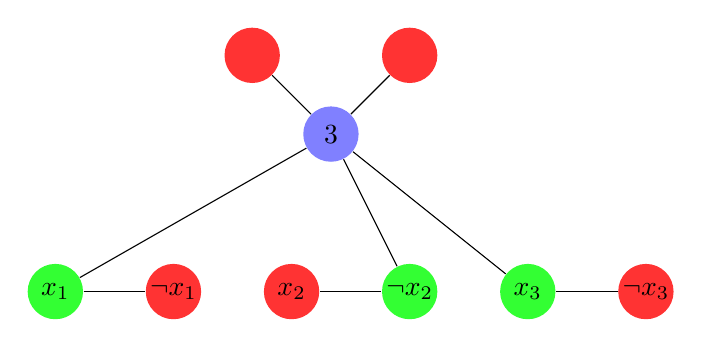
\begin{tikzpicture}
			\node[vertex, fill = red!80] (s1)  at (1,4)  {};
			\node[vertex, fill = red!80] (s2)  at (3,4)  {};
			\node[vertex,fill = blue!50] (s3)  at (2,3)  {3};
			
			\node[vertex, fill = green!80] (x1) at(-1.5,1) {$x_1$};
			\node[vertex, fill = red!80] (x1') at(0,1) {$\neg x_1$};
			\node[vertex,fill = red!80] (x2) at (1.5,1) {$x_2$};
			\node[vertex, fill = green!80] (x2') at (3,1) {$\neg x_2$};
			\node[vertex, fill = green!80] (x3) at (4.5,1) {$x_3$};
			\node[vertex,fill = red!80] (x3') at (6,1) {$\neg x_3$};
			\draw (s1) -- (s3);
			\draw (s2) -- (s3);
			\draw (s3) -- (x1);
			\draw (s3) -- (x2');
			\draw (s3) -- (x3);
			\draw (x1) -- (x1');
			\draw (x2) -- (x2');
			\draw (x3) -- (x3');
			\end{tikzpicture}
		\end{center} 	
	we can not color the nodes to make sure that blue node $3$ has exactly $3$ neighboring nodes containing mines.
	Thus $3-SAT \leq_p mine-consistency$
\end{itemize}
Hence $mine-consistency$ is in NP-complete.
 